% !TeX program = pdflatex
% =============================================================================
% Zusammenfassung: Lorentzkraft Teil 1 -- die drei Experimente und ihre
% Kernerkenntnisse
% UZH Praktikum I -- Sara Romer Urban, Kantonsschule im Lee, HS2026
% Klassen: 4fh (15.09.2026) + 4cdeg (18.09.2026) -- gemeinsames Material
%
% Anders als eine erste Fassung dieses Dokuments ist dies KEIN
% Protokoll-/Aufgaben-Dokument mehr (Experimente und Aufgaben leben im
% Arbeitsblatt, arbeitsblatt6-lorentzkraft-teil1.tex) -- stattdessen ein
% fertiges, durchgehend ausformuliertes Zusammenfassungsdokument der drei im
% Unterricht gezeigten Experimente (Leiterschaukel, zwei parallele Leiter,
% Fadenstrahlrohr) samt der daraus gewonnenen Kernerkenntnisse, gedacht zur
% Pruefungsvorbereitung (Nachschlagen/Repetieren, keine Luecken zum
% Ausfuellen).
%
% Quellen: siehe arbeitsblatt6-lorentzkraft-teil1.tex und lernziele.md
% (dieser Ordner) sowie literatur/ (PhysikLibre Kap. 13.5, LEIFIphysik
% "LORENTZ-Kraft"/"Fadenstrahlrohr"). Bilder: siehe Bilder/*.pdf
% (SVG->PDF via Inkscape) und Bilder/*.jpg.
% =============================================================================
\documentclass[11pt,a4paper]{exam}

\usepackage[T1]{fontenc}
\usepackage[utf8]{inputenc}
\usepackage[ngerman]{babel}
\usepackage{lmodern}
\usepackage[a4paper,margin=2.2cm,headheight=14pt]{geometry}
\usepackage{amsmath}
\usepackage{amssymb}
\usepackage{siunitx}
% Hausstil: zusammengesetzte Einheiten immer als echter Bruch (\frac), nicht
% als Inline-Schrägstrich oder \tfrac -- gilt global für jedes \si/\SI.
\sisetup{per-mode=fraction,fraction-command=\frac}
\usepackage{array,booktabs,tabularx,multirow}
\usepackage{enumitem}
\usepackage{xcolor}
\usepackage{colortbl}
\usepackage{tikz}
\usepackage{physics}
\usepackage{circuitikz}
\usepackage[most]{tcolorbox}
\usepackage{lastpage}
\usepackage{graphicx}
\usepackage{hyperref}

\usetikzlibrary{arrows.meta,calc,angles,quotes,decorations.markings}

\usepackage{setspace}
\usepackage{needspace}
\setlength{\parindent}{0pt}
\setlength{\parskip}{0.6em}
\setstretch{1.08}
\setlist[itemize]{itemsep=0.4em}

% -----------------------------
% Farben (Corporate-Farbschema Physik KFR)
% -----------------------------
\definecolor{titleblue}{HTML}{183A6B}
\definecolor{accentblue}{HTML}{2E6F9E}
\definecolor{lightblue}{HTML}{EAF4FB}
\definecolor{verylightblue}{HTML}{F7FBFE}
\definecolor{lightgray}{HTML}{F4F6F8}
\definecolor{darkgray}{HTML}{4A4A4A}
\definecolor{accentorange}{HTML}{D9720C}
\definecolor{accentpurple}{HTML}{7B2D8E}
\definecolor{theorygreen}{HTML}{2E7D4F}
\definecolor{lighttheorygreen}{HTML}{EAF7EF}
\definecolor{groupteal}{HTML}{1B7F72}
\definecolor{lightgroupteal}{HTML}{E8F5F3}
\definecolor{lightorange}{HTML}{FCEEE0}
\definecolor{lightpurple}{HTML}{F3EAF7}

\hypersetup{
  colorlinks=true,
  urlcolor=accentblue,
  linkcolor=accentblue,
  pdftitle={Zusammenfassung: Lorentzkraft (Teil 1)},
  pdfauthor={Loris Keller}
}

% -----------------------------
% Boxen (Praktikum I: siehe institutionen/UZH-Praktikum-I/CLAUDE.md,
% Abschnitt "Boxen-Layout" -- nur Formel- und Hinweisbox bleiben farbig,
% dieses Dokument braucht keine Antwortbox, da es keine Luecken enthält.)
% -----------------------------
\tcbset{before skip=10pt, after skip=10pt}
\newtcolorbox{titlebox}{
  enhanced,
  colback=titleblue,
  colframe=titleblue,
  boxrule=0pt,
  arc=3mm,
  left=3mm,right=3mm,top=3mm,bottom=3mm
}

\newenvironment{theoriebox}[1][Theorie]{%
  \par\addvspace{10pt}\noindent\textbf{#1}\par\smallskip\noindent
}{%
  \par\addvspace{10pt}
}

\newenvironment{beispielbox}[1][Beispiel]{%
  \par\addvspace{10pt}\noindent\textbf{#1}\par\smallskip\noindent
}{%
  \par\addvspace{10pt}
}

\newtcolorbox{hinweisbox}[1][Hinweis]{
  enhanced,
  breakable,
  colback=lightorange,
  colframe=accentorange,
  title={#1},
  fonttitle=\bfseries,
  boxrule=0.7pt,
  arc=2mm,
  left=5mm,right=5mm,top=2mm,bottom=2mm
}

\newtcolorbox{formelbox}[1][Formel]{
  enhanced,
  breakable,
  colback=lightpurple,
  colframe=accentpurple,
  title={#1},
  fonttitle=\bfseries,
  boxrule=0.9pt,
  arc=2mm,
  left=5mm,right=5mm,top=2mm,bottom=2mm
}

\pagestyle{headandfoot}
\cfoot{\textcolor{darkgray}{Seite \thepage\ von \pageref{LastPage}}}

\newcommand{\Kopfzeile}[4]{%
  \begin{titlebox}
    {\color{white}\sffamily\bfseries\Large #4}
  \end{titlebox}
  \vspace{0.5em}
  \noindent\textbf{Klasse:}~#1 \hfill \textbf{Datum:}~#2 \hfill \textbf{Thema:}~#3
    \hfill \textbf{Lehrperson:}~Loris Keller
  \vspace{0.8em}
  \lhead{\textcolor{darkgray}{#3}}
  \rhead{\textcolor{darkgray}{#4}}
}

% Werte für Kopfzeile zentral setzen
\newcommand{\Klasse}{4fh / 4cdeg (SP4)}
\newcommand{\Datum}{15.09.2026 (4fh) / 18.09.2026 (4cdeg)}
\newcommand{\Thema}{Lorentzkraft (Teil 1)}
\newcommand{\DokumentTitel}{Zusammenfassung: Lorentzkraft (Teil 1)}

\begin{document}

\Kopfzeile{\Klasse}{\Datum}{\Thema}{\DokumentTitel}

\noindent Dieses Dokument fasst die drei im Unterricht gezeigten Experimente
und die daraus gewonnenen Kernerkenntnisse zusammen -- zum Nachschlagen und
zur Prüfungsvorbereitung. Herleitungen und Übungsaufgaben finden Sie im
Arbeitsblatt.

% =============================================================================
% Experiment 1: Leiterschaukel
% =============================================================================
\begin{theoriebox}[Experiment 1: Leiterschaukel]
\textbf{\emph{Aufbau und Beobachtung.}} Ein lose aufgehängter,
schaukelförmiger Leiter befindet sich zwischen den Polen eines
Hufeisenmagneten; der Stromkreis lässt sich einschalten und umpolen.
Schaltet man den Strom ein, schlägt die Schaukel seitlich aus. Polt man
\emph{nur} den Strom oder \emph{nur} den Magneten um, kehrt sich die
Auslenkungsrichtung um. Polt man \emph{beide} zugleich um, zeigt die
Schaukel wieder in die ursprüngliche Richtung.
\begin{center}
  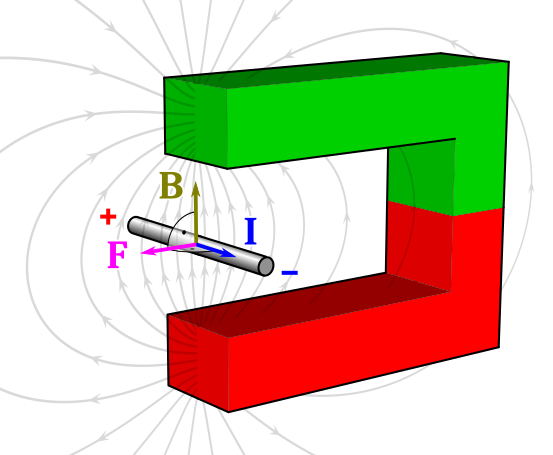
\includegraphics[width=6.5cm]{Bilder/leiterschaukel-experiment-preview.pdf}
\end{center}
{\scriptsize Leiterschaukel im Feld eines Hufeisenmagneten: Stromrichtung
$I$, Feldrichtung $B$, resultierende Kraft $F$ auf den Leiter.}

\textbf{\emph{Kernerkenntnis.}} Ein stromdurchflossener Leiter in einem
externen Magnetfeld $B$ (also einem Feld, das nicht vom Strom selbst
erzeugt wird) erfährt die \textbf{\emph{magnetische Kraft}}
\begin{formelbox}[Magnetische Kraft]
\[
  \vec F = I\,\vec l\times\vec B, \qquad F = I\cdot l\cdot B\cdot\sin\alpha
\]
Einheit: $\si{\newton}$. Im rechtwinkligen Spezialfall ($\vec I\perp\vec
B$, $\alpha=90^\circ$) vereinfacht sich das zu $F=I\cdot l\cdot B$.
\end{formelbox}
Die Richtung von $F$ liefert die \textbf{\emph{Drei-Finger-Regel der
rechten Hand}} (Daumen = Stromrichtung $I$, Zeigefinger = Feldrichtung
$B$, Mittelfinger = Kraftrichtung $F$ -- alle drei paarweise senkrecht
zueinander). Kehrt man nur $I$ oder nur $B$ um, dreht sich damit auch $F$
um; kehrt man beide gleichzeitig um, bleibt die relative Anordnung der
drei Richtungen gleich, und $F$ zeigt wieder in die ursprüngliche
Richtung -- genau das erklärt die Beobachtung an der Leiterschaukel.
\begin{center}
  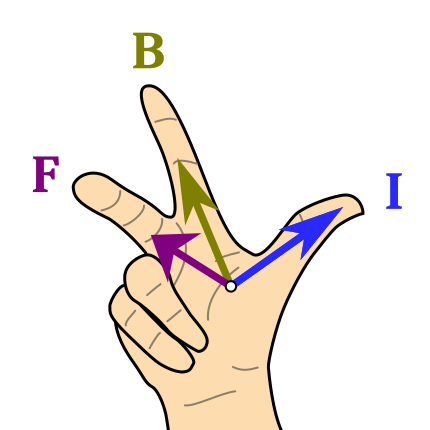
\includegraphics[width=5cm]{Bilder/uvw-regel-strom.pdf}
\end{center}
{\scriptsize Daumen = Stromrichtung $I$, Zeigefinger = Feldrichtung $B$,
Mittelfinger = Kraftrichtung $F$.}
\end{theoriebox}

% =============================================================================
% Experiment 2: Zwei parallele Leiter
% =============================================================================
\begin{theoriebox}[Experiment 2: Zwei parallele Leiter]
\textbf{\emph{Aufbau und Beobachtung.}} Zwei parallel hängende,
stromdurchflossene Drähte, deren Stromrichtung sich unabhängig voneinander
umpolen lässt, wurden im Plenum gezeigt: Bei \textbf{gleichgerichteten}
Strömen ziehen sich die Drähte an, bei \textbf{entgegengesetzt}
gerichteten Strömen stossen sie sich ab.
\begin{center}
  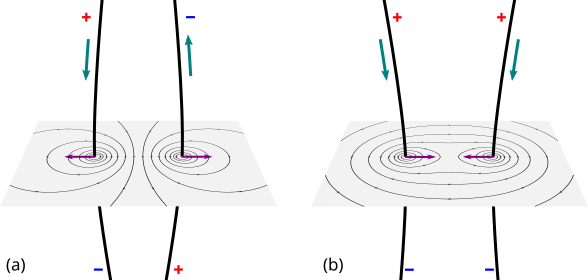
\includegraphics[width=8cm]{Bilder/antiparallel-and-parallel-wires.pdf}
\end{center}
{\scriptsize Links (a): entgegengesetzte Ströme, Abstossung. Rechts (b):
gleichgerichtete Ströme, Anziehung.}

\textbf{\emph{Kernerkenntnis.}} Jeder der beiden Leiter erzeugt sein
eigenes Magnetfeld (bereits aus Magnetfelder bekannt: $B=\frac{\mu_0}{2\pi}
\cdot\frac{I}{r}$) und befindet sich damit gleichzeitig im Feld des jeweils
anderen. Kombiniert man diese Feldformel mit der magnetischen Kraft
$F=IlB$, ergibt sich das \textbf{\emph{Ampère'sche Kraftgesetz}}:
\begin{formelbox}[Kraft zwischen zwei parallelen Leitern]
\[
  \frac{F}{l} = \frac{\mu_0}{2\pi}\cdot\frac{I_1\cdot I_2}{r}, \qquad
  \text{Einheit von }\frac{F}{l}\colon\ \si{\newton\per\meter}
\]
\end{formelbox}
\begin{center}
  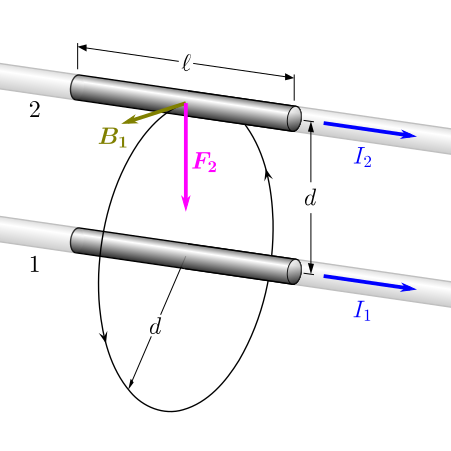
\includegraphics[width=6.5cm]{Bilder/amperes-force-law.pdf}
\end{center}
{\scriptsize Das Feld $B_1$ des unteren Leiters wirkt am Ort des oberen
Leiters und erzeugt dort die Kraft $F_2$ auf ein Leiterstück der Länge
$l$.}

Die \textbf{\emph{Richtung}} dieser Kraft ergibt sich, indem man wieder
die Drei-Finger-Regel auf eine einzelne bewegte Ladung im einen Leiter
anwendet, die sich im Feld des anderen Leiters befindet: Fliessen die
Ströme \textbf{gleichgerichtet}, zeigt die Kraft zum jeweils anderen
Leiter hin (\textbf{Anziehung}); fliessen sie \textbf{entgegengesetzt},
zeigt sie vom anderen Leiter weg (\textbf{Abstossung}).
\begin{center}
  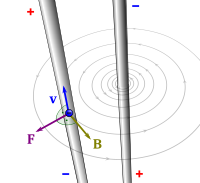
\includegraphics[width=5cm]{Bilder/anti-parallel-currents-magnetic-force.pdf}
\end{center}
{\scriptsize Eine einzelne (positive) Ladung im rechten Leiter, bewegt im
Feld $B$ des linken Leiters -- die Drei-Finger-Regel liefert die Kraft
$F$.}
Achtung, Verwechslungsgefahr mit Polen/Ladungen: Dort gilt \glqq gleich
stösst ab\grqq{} -- bei parallelen Strömen gilt das Gegenteil. Genau
dieser Aufbau diente vor der SI-Neudefinition 2019 direkt zur Definition
der Einheit Ampere.
\end{theoriebox}

% =============================================================================
% Experiment 3: Fadenstrahlrohr
% =============================================================================
\begin{theoriebox}[Experiment 3: Fadenstrahlrohr]
\textbf{\emph{Aufbau und Beobachtung.}} Im Fadenstrahlrohr werden
Elektronen in einer Elektronenkanone durch eine Beschleunigungsspannung
$U_B$ auf eine Geschwindigkeit $v$ gebracht und treten dann in ein
(näherungsweise homogenes) Magnetfeld $B$ senkrecht zu $v$ ein. Die
Elektronen selbst sind unsichtbar; ihre Bahn wird erst durch das
verdünnte Restgas im Rohr als leuchtende Spur sichtbar. Beim Einschalten
des Feldes läuft diese Spur auf einer \textbf{geschlossenen Kreisbahn}.
\begin{center}
  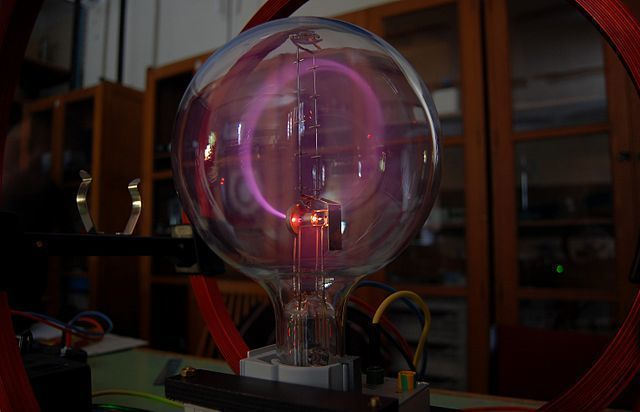
\includegraphics[width=6cm]{Bilder/beam-of-electrons.jpg}
\end{center}
{\scriptsize Echtes Fadenstrahlrohr: die leuchtende Elektronenspur ist
zwischen den Helmholtzspulen sichtbar.}

\textbf{\emph{Kernerkenntnis.}} Die Lorentzkraft wirkt nicht nur auf
Ladungen im Leiter, sondern auf jede bewegte Ladung -- auch auf eine
\textbf{freie} Ladung wie ein einzelnes Elektron:
\begin{formelbox}[Lorentzkraft]
\[
  \vec F = q\,\vec v\times\vec B, \qquad F = q\cdot v\cdot B\cdot\sin\alpha
\]
Einheit: $\si{\newton}$. Im rechtwinkligen Spezialfall ($\vec v\perp\vec
B$) vereinfacht sich das zu $F=q\cdot v\cdot B$.
\end{formelbox}
Da die Lorentzkraft stets \textbf{senkrecht} zur Geschwindigkeit $v$
steht, ändert sie nur die Bewegungs\emph{richtung}, nie den
Geschwindigkeits\emph{betrag} -- genau das ist die Bedingung für eine
\textbf{\emph{Zentripetalkraft}} aus der Mechanik. Die Lorentzkraft wirkt
hier also als Zentripetalkraft und hält die Elektronen auf ihrer
Kreisbahn. Die Krümmungsrichtung folgt aus der \textbf{linken}
Hand-Variante der Drei-Finger-Regel (Elektronen sind negativ geladen):
Daumen in Richtung $v$, Zeigefinger in Richtung $B$, Mittelfinger zeigt
zum Kreismittelpunkt.
\begin{center}
\begin{tikzpicture}[>=Latex,scale=1.1]
  \begin{scope}
    \clip (0,0) circle (2.2);
    \foreach \x in {-2,-1.3,-0.6,0.1,0.8,1.5,2.2}{
      \foreach \y in {-2,-1.3,-0.6,0.1,0.8,1.5,2.2}{
        \node[font=\small] at (\x,\y) {$\otimes$};
      }
    }
  \end{scope}
  \draw[thick] (0,0) circle (2.2);
  \draw[thick,-{Latex[length=3mm]}] (-3.7,0) -- (-2.2,0);
  \node[align=center] at (-3.7,0.35) {\scriptsize $e^-$, $v$};
  \draw[thick,purple] (-2.2,-1.3) circle (1.3);
  \filldraw[purple] (-2.2,-1.3) circle (1.2pt);
  \draw[thick,-{Latex[length=2.5mm]},purple] (-2.2,0) -- (-2.2,-1.1) node[midway,left]{\scriptsize $F_L$};
\end{tikzpicture}
\end{center}
{\scriptsize Draufsicht, $\otimes$ = Magnetfeld $B$ ins Blatt hinein: die
Lorentzkraft $F_L$ zeigt stets zum Kreismittelpunkt und hält die
Elektronen auf der Kreisbahn.}
In Teil 2 wird diese Kreisbahn quantitativ vertieft: Wovon hängt ihr
Radius $r=\frac{m\cdot v}{q\cdot B}$ genau ab?
\end{theoriebox}

% =============================================================================
% Formelübersicht
% =============================================================================
\begin{formelbox}[Formelübersicht Lorentzkraft Teil 1]
\begin{tabularx}{\linewidth}{@{}p{4.6cm}X@{}}
\textbf{Magnetische Kraft} & $F = I\cdot l\cdot B\cdot\sin\alpha$, Spezialfall $\vec I\perp\vec B$: $F=I\cdot l\cdot B$ \\[0.4em]
\textbf{Lorentzkraft} & $F = q\cdot v\cdot B\cdot\sin\alpha$, Spezialfall $\vec v\perp\vec B$: $F=q\cdot v\cdot B$ \\[0.4em]
\textbf{Ampère'sches Kraftgesetz} & $\dfrac{F}{l} = \dfrac{\mu_0}{2\pi}\cdot\dfrac{I_1\cdot I_2}{r}$ \\[0.6em]
\textbf{Richtung} & Drei-Finger-Regel: Daumen = Strom-/Geschwindigkeitsrichtung, Zeigefinger = Feldrichtung, Mittelfinger = Kraftrichtung. Rechte Hand für positive, linke Hand für negative Ladungsträger. \\
\end{tabularx}
\end{formelbox}

\end{document}
